\section{Introduction}
It is the main goal of this experiment to investigate the mode of operation of an operational amplifier and to compare the results with the ideal model of this device

\section{Theory}
\FloatBarrier
\begin{figure}
  \centering
  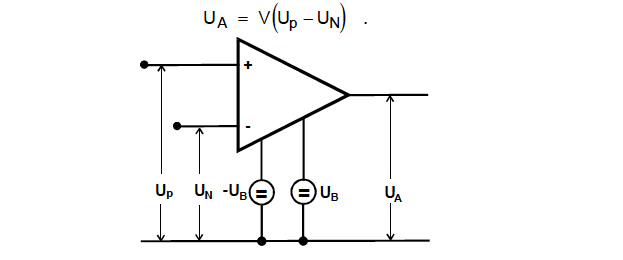
\includegraphics[scale=0.5]{opamp.PNG}
  \caption{Circuit of an operational amplifier. \cite{Q1}}
  \label{abb1}
\end{figure}
\FloatBarrier
The picture above shows the circuit of an ideal operational amplifier. It is
fed with two constant voltages $U_{\text{B}}$ and -$U_{\text{B}}$.
Further the operational amplifier has two inputs, an inverting ($-$) and a
non-inverting ($+$) one. The output voltage $U_{\text{A}}$ is calculated by:
\begin{align}
    U_{\text{A}} = V(U_{\text{p}}-U_{\text{N}}) \ .
    \label{eq:outputvoltage}
\end{align}
Where $U_{\text{p}}$ represents the voltage going into the non-inverting ,
$U_{\text{N}}$ the one going into the inverting input and $V$, the proportionality
factor is the open loop gain of the operational amplifier.
The output voltage can only swing within the following range:
\begin{align*}
    -U_{\text{B}} < U_{\text{A}} < U_{\text{B}} \ .
\end{align*}
Outside of this interval the output voltage $U_{\text{A}}$ equals the operational
voltage $\pm U_{\text{B}}$ and the operational amplifier is in a saturation
condition. Within the intervall the amplification can be described as
linear.
The saturation curve can be seen in the figure \ref{abb2}. It has to be said that this is a graphic demonstration in which the gradient of the straight line is pictured excessively low.

\FloatBarrier
\begin{figure}
  \centering
  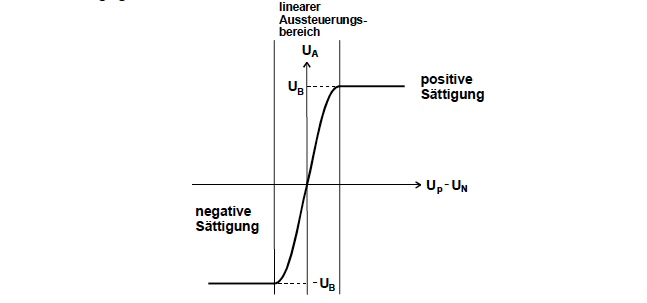
\includegraphics[scale=0.5]{saturation.PNG}
  \caption{Characteristic curve of an operational amplifier. \cite{Q1}}
  \label{abb2}
\end{figure}
\FloatBarrier

\noindent In order to describe an operational amplifier correctly it is important to define
a few more parameters such as the two input resistances $r_{\text{e}_{{}_\text{p}}}$
and $r_{\text{e}_{{}_\text{N}}}$ and the output resistance $r_{\text{a}}$.
Usually the open loop gain $V$ is very high and dependent on the frequency of the
input voltage, in the case of an ideal operational amplifier it is considered to
be infinite. The same applies to the two input resistances. They are usually very
high and are considered to be infinite when talking about the ideal operational
amplifier. The output resistance is to be kept as small as possible which is why
it is considered to be zero for the ideal case.
\begin{align*}
    V_{\text{id}}=\infty,~ r_{\text{e}_{\text{id}}}=\infty,~ r_{\text{a}_{\text{id}}}=0
\end{align*}
Regarding a real operational amplifier some assymetrics in the amplifying inputs
have to be taken into consideration which is why the output voltage is unequal to
zero even when the two input voltages $U_{\text{Gl}}$ are the same. This is
called the common mode gain. In this case the common mode amplification is described
as:
\begin{align*}
    V_{\text{Gl}}:=\frac{\Delta U_{\text{A}}}{\Delta U_{\text{Gl}}}.
\end{align*}
Due to the fact that the real input resistances cannot be infinite there will occur
input currents, $I_{\text{p}}$ and $I_{\text{N}}$, that are unequal to zero.
The overall input current is described as follows:
\begin{align*}
    I_{\text{B}} = \frac{1}{2} \left( I_{\text{p}} + I_{\text{N}} \right).
\end{align*}
Further the difference betweeen the two input currents is called offset current
and can be described as:
\begin{align*}
    I_0:=I_{\text{p}} - I_{\text{N}} ,~ \text{ with } U_{\text{N}} = U_{\text{p}} = 0 .
\end{align*}
With the two input currents $I_{\text{p}}$ and $I_{\text{N}}$ it is now possible
to calculate the differential input impedance:
\begin{align*}
    r_\text{D}:=
	\begin{cases}
		\frac{\Delta U_{\text{p}}}{\Delta I_{\text{p}}} ~ \text{, while }~ U_{\text{N}} = 0   \\
		\\
		\frac{\Delta U_{\text{N}}}{\Delta I_{\text{N}}} ~ \text{, while }~ U_\text{p}=0
\end{cases}
\end{align*}
As well as the common mode input impedance:
\begin{align*}
    r_{\text{Gl}} = \frac{\Delta U_{\text{Gl}}}{\Delta I_{\text{Gl}}}
\end{align*}
In this equation $U_{\text{Gl}}$ is equal to $U_{\text{p}}$ and $U_{\text{N}}$ and
$I_{\text{Gl}}$ is calculated by the addition of $I_{\text{p}}$ and $I_{\text{N}}$.

\noindent For a real operational amplifier the output voltage is often unequal to zero while
$U_{\text{p}} = U_{\text{N}} = 0$, eventhough this could be concluded from equation
\ref{eq:outputvoltage}.
Therefore an offset voltage $U_0$ is defined as the voltage difference that has to
be set between the two input voltages so the output voltage dissapears:
\begin{align*}
    U_0 := U_{\text{p}} - U_{\text{N}} ,~ \text{ for } U_{\text{A}}=0
\end{align*}
All the above currents and voltage dissapear in the case of the ideal operational
amplifier and the impedances $r_{\text{D}}$ and $r_{\text{Gl}}$ are considered to
be infinite.

\subsection{Linear inverting amplifier}
Due to the already mentioned very high open loop gain $V$ it is impossible to use
an operational amplifier as a linear amplifier without making any modifications to
the circuit. The modified circuit is displayed in figure \ref{abb3}. The difference
to figure \ref{abb1} is the feedback network which puts a part of the output
voltage back to the inverting input. This leads to a decrease of the input voltage $U_{\text{N}}$, being $U_{\text{A}}$ opposite in sign with respect to $U_{1}$.
\FloatBarrier
\begin{figure}
  \centering
  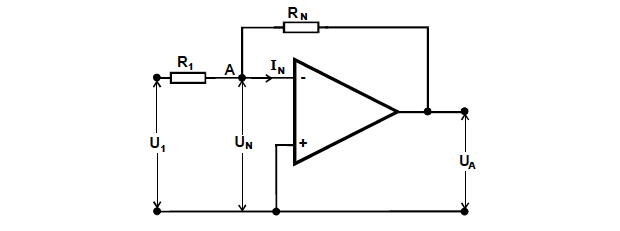
\includegraphics[scale=0.5]{degenerative.PNG}
  \caption{Circuit of the linear inverting amplifier. \cite{Q1}}
  \label{abb3}
\end{figure}
\FloatBarrier
The high value for the open loop gain is also the reason for the fact that the
voltage that goes into the inverting input is approxiamtely zero:
\begin{align*}
    U_{\text{N}} = - \frac{U_{\text{A}}}{V}
\end{align*}
as well as the input current $I_{\text{N}}$ because the input impedance is extremely
high.
In the circuit shown in figure \ref{abb3} the amplification factor $V^{\prime}$ for an ideal
oerational amplifier with this feedback network, can be calculated according to the Kirchhoff Current Law
applied to point A in the figure:
\begin{align}
    V'=-\frac{\text{R}_{\text{N}}}{\text{R}_1}.
    \label{eq:ampfactor}
\end{align}
In order to calculate the amplification factor $V'$ for a real operational amplifier
the following equation is used:
\begin{align}
    \frac{1}{V'} \approx \frac{1}{V} + \frac{\text{R}_1}{\text{R}_{\text{N}}}
    \label{eq:ampfactor_real}
\end{align}
Taking a look at the equation \ref{eq:ampfactor_real} it can be seen that $V'$ has
the same value in \ref{eq:ampfactor} as in \ref{eq:ampfactor_real} in the case of
$R_{\text{N}}/R_1 \ll V$.
The fact that the amplification $V'$ is modified by the outer resistance and the
relation between $R_{\text{N}}$ and $\text{R}_1$ makes the amplifier less sensitive to
external factors such as temperature which could influence $V$.
Therefore by including the negative feedback into the circuit the linear amplifier becomes
much more stable.
At the same time the output resistance $r_{\text{a}}$ is decreased by the factor
of $g$:
\begin{align*}
    g:= \frac{V}{V'}.
\end{align*}
The influence of possible variations in the open loop gain on the amplification
factor $V'$ are also reduced by the factor $g$:
\begin{align*}
    \frac{\Delta V'}{V'}=\frac{1}{g}\frac{\Delta V}{V}.
\end{align*}
Finally the bandwidth of the operational amplifier is broadened by the factor of
$g$ which means that higher frequencies are transmitted wihtout distortion as shown
in figure \ref{abb4}. The highest frequency that is transmitted without distortion
is called cut off frequency. The amplification factor $V'$ has decreased to a value of
1 and the amplifier does not show a linear behaviour anymore.
\FloatBarrier
\begin{figure}
  \centering
  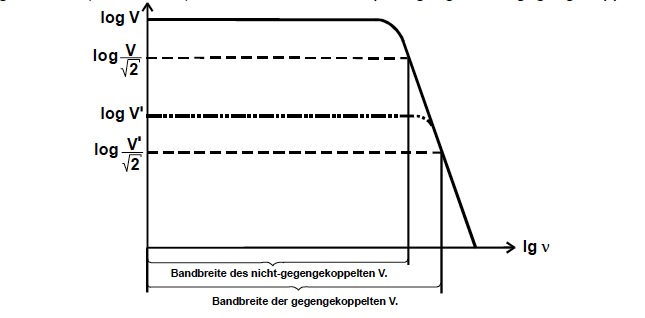
\includegraphics[scale=0.5]{bandwidth.PNG}
  \caption{Frequency response of an operational amplifier. \cite{Q1}}
  \label{abb4}
\end{figure}
\FloatBarrier

\subsection{Reverse Integrator}
If the feedback resistance in the circuit shown in \ref{abb3} is replaced by a capacitor \textbf{C}
as shown in \ref{abb5} the operational amplifier can be used as a reverse integrator
of the input signal so the output signal can be calculated by:
\begin{align}
    U_{\text{A}} = -\frac{1}{\text{RC}} \int U_1(t) dt
    \label{eq:U_A}
\end{align}
The '-' in the formula \ref{eq:U_A} is the reason for the integrator being called a reverse
integrator and $U_{\text{N}} \approx 0$.
In case of a sinusodial input ($U_{1}=U_0 sin(\omega t)$) of frequency \omega the output voltage depends on the inverse frequency
of the input voltage.
\FloatBarrier
\begin{figure}
  \centering
  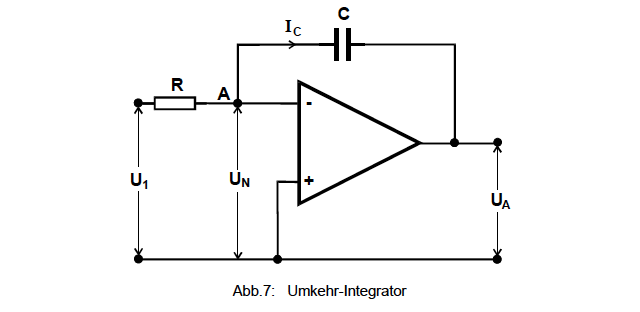
\includegraphics[scale=0.5]{integrator.PNG}
  \caption{Circuit of a reverse integrator. \cite{Q1}}
  \label{abb5}
\end{figure}
\FloatBarrier

\section{Experimental set-up}
The circuits that are previously described can be easily built up on a bread
board. The operational amplifier being used in the experient is a LMRS1, a
collection of resistors and capacitors were used for the realization of the
circuits.\\
input voltage wavefronts were generated by means of a signal generator, input
and output time dependent signals were measured with an agilent oscilloscope.
Constant voltages, as well as resistor and capacitor values were measured
with a digital multimeter.

\section{Lead-through}

In the first part of the experiment the circuit from figure \ref{abb3} is used to
figure out the characteristic roll off and although the cut-off frequency of the
operational amplifier . A constant supply voltage of the operational
amplifier of $\pm \SI{12}{\volt}$ has to be guaranteed for each part of the experiment.
As soon as the circuit from figure \ref{abb3} is set up the frequency of an input
sine-voltage is increased from $\SI{10}{\hertz}$ up to $\SI{1}{\mega \hertz}$ for
two different ratios of the feedback network resistances.
The second part of the experiment includes the circuit of the reverse integrator as
shown in figure \ref{abb5}. In the first subsection the qualitative behaviour of the integrator is shown by a simple comparison of the input and output waveforms.
Afterwards the frequency of a sinusodial input voltage is increased from $\SI{570}{\hertz}$
to $\SI{16}{\kilo \hertz}$ in order to verify the relationship of equation \ref{eq:U_A}.

\section{Analysis}

The data of the first two measurements are written in the table \ref{tab:1}. In
figures \ref{abb:1} and \ref{abb:2} you can see the data on logarithmic scales
together a linear regression of the form
\begin{equation*}
  ln(U) = a \cdot ln(\nu) + b
\end{equation*}
best fit results are

\begin{align*}
  a_1 &= \num{-0.783(25)} \\
  b_1 &= \num{10.53(30)} \\
\end{align*}
and
\begin{align*}
  a_2 &= \num{-0.760(12)} \\
  b_2 &= \num{11.32(13)} \\
\end{align*}

The critical frequency $\nu_g$ is defined as the frequency, when the amplification drops
to $\frac{V_0}{\sqrt{2}}$.
\begin{align*}
  \nu_{\symup{g,1}} = \SI{0.44(22)}{\mega\hertz} \\
  \nu_{\symup{g,2}} = \SI{0.62(17)}{\mega\hertz}
\end{align*}

The normal amplification $V_0$ can be calculated with the arithmetic mean of
the first data. In the ideal case this value is set by ... ?

\begin{align*}
  V_{0, 1} = 7.612 \\
  V_{0, 2} = 99.302
\end{align*}

The product of the normal amplification $V_0$ and the critical frequency should
be a constant:
\begin{align*}
  V_{0, 1} \cdot \nu_{\symup{g,1}} = \SI{0.9(5)}{\mega\hertz} \\
  V_{0, 2} \cdot \nu_{\symup{g,2}} = \SI{2.9(8)}{\mega\hertz}
\end{align*}



\begin{table}
  \centering
  \caption{Data of the characteristic roll off and the cut-off frequency.}
  \label{tab:1}
  \begin{tabular}{c c | c c}
    \toprule
    \multicolumn{2}{c}{measurement 1} & \multicolumn{2}{c}{measurement 2} \\
    $\nu$ / \si{\hertz} & $U$ / \si{\milli\volt} & $\nu$ / \si{\hertz} & $U$ / \si{\volt} \\
    \midrule
    10      &  62  &  10     &  5.75 \\
    50      &  61  &  100    &  5.75 \\
    100     &  60  &  500    &  5.67 \\
    200     &  61  &  1000   &  5.67 \\
    500     &  61  &  2500   &  5.03 \\
    1000    &  61  &  5000   &  5.03 \\
    2500    &  62  &  6000   &  4.90 \\
    5000    &  61  &  7000   &  4.82 \\
    7500    &  61  &  8000   &  4.50 \\
    10000   &  59  &  9000   &  4.38 \\
    15000   &  60  &  10000  &  4.18 \\
    20000   &  59  &  11000  &  4.02 \\
    25000   &  59  &  12000  &  3.82 \\
    30000   &  59  &  13000  &  3.66 \\
    35000   &  58  &  14000  &  3.5  \\
    45000   &  57  &  15000  &  3.3  \\
    50000   &  55  &  16000  &  3.18 \\
    60000   &  53  &  17000  &  3.06 \\
    70000   &  50  &  18000  &  2.93 \\
    80000   &  47  &  20000  &  2.69 \\
    90000   &  43  &  22500  &  2.45 \\
    100000  &  40  &  25000  &  2.25 \\
    125000  &  35  &  30000  &  1.93 \\
    150000  &  29  &  35000  &  1.69 \\
    175000  &  24  &  40000  &  1.53 \\
    250000  &  18  &  45000  &  1.37 \\
    300000  &  15  &  50000  &  1.25 \\
    400000  &  12  &  60000  &  1.05 \\
    500000  &  9   &  70000  &  0.920 \\
    600000  &  9   &  80000  &  0.800 \\
    1000000 &  6   &  100000 &  0.68  \\
            &      &  150000 &  0.520 \\
            &      &  300000 &  0.320 \\
            &      &  450000 &  0.280 \\
    \bottomrule
  \end{tabular}
\end{table}

\begin{figure}
  \centering
  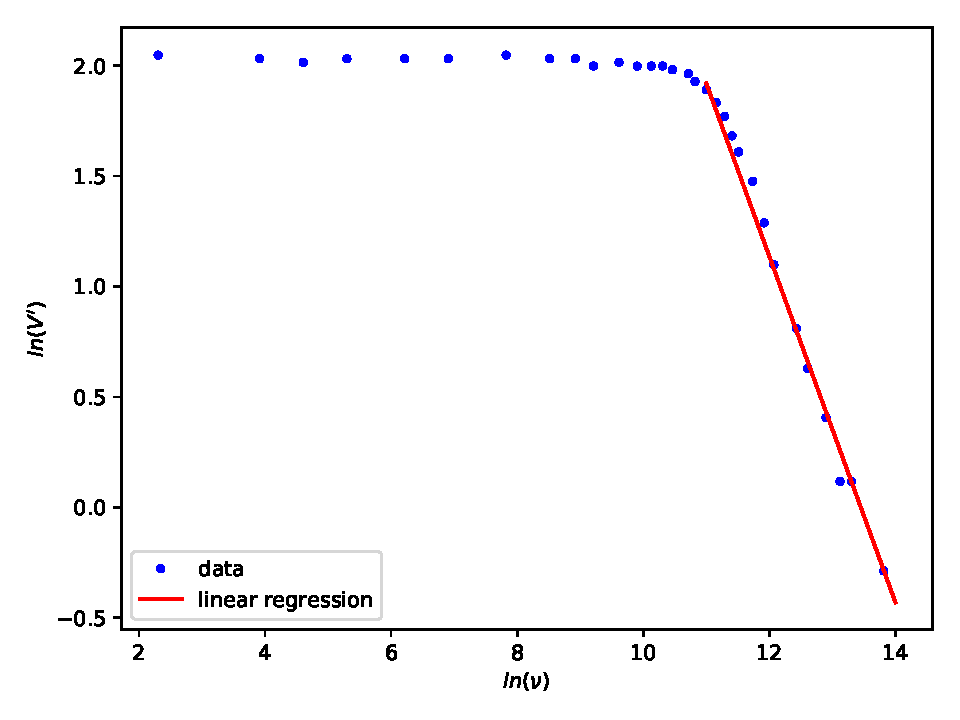
\includegraphics[scale=0.7]{A1.pdf}
  \caption{First measurement with linear regression.}
  \label{abb:1}
\end{figure}
\begin{figure}
  \centering
  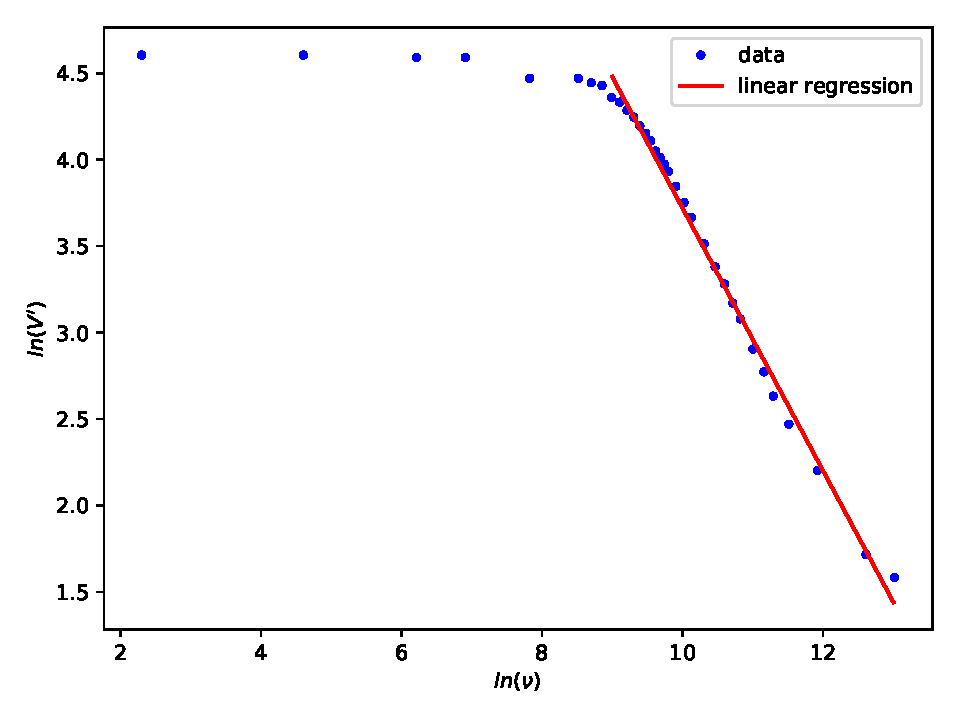
\includegraphics[scale=0.7]{A2.pdf}
  \caption{Second measurement with linear regression.}
  \label{abb:2}
\end{figure}

\subsection{Reverse Integrator}
In figure \ref{abb:3} you can see the integral of a square-wave-voltage and in
figure \ref{abb:4} the integral of a triangle-oscillation.
The green line represents the function and the yellow line the integral of
the function.

The data of the voltage amplitude as a function of the frequency is written
in the table \ref{tab:2} and shown in \ref{abb:5}. To analyse the porportionality of the voltage amplitude
in function of the inverse frequency or rather the inverse of the phase velocity,
you have to do a linear regression:
\begin{equation*}
  \frac{U}{U_0} = a_2 \cdot \frac{1}{\omega} + b_2 = a_2 \cdot \frac{1}{2 \pi \nu} + b_2
\end{equation*}
$a_2$ and $b_2$ are regression parameter, with the values
\begin{align*}
  a_3 &= \SI{1.413(8)e5}{\per\second} \\
  b_3 &= \SI{0.75(10)}{} \\
\end{align*}
You can calculate the value of $RC$ by comparing the slope with the formula
\begin{equation}
  \label{eq:1}
  U = \frac{U_0}{\omega R C} \cos{(\omega t)}
\end{equation}
\begin{equation*}
  RC = \SI{7.08(4)e-6}{\second}
\end{equation*}
Compared with the theoretical value of $RC_{theory}= \SI{6.15e-6}{\second}$, we measured before,  there is a
deviation of $\SI{15}{\percent}$.
\begin{table}
  \centering
  \caption{The data of the ouput voltage in function of the frequency.}
  \label{tab:2}
  \begin{tabular}{c c| c c}
    \toprule
    $\nu$ / \si{\hertz} & $U$ / \si{\volt} & $\nu$ / \si{\hertz} & $U$ / \si{\volt} \\
    \midrule
    570  & 23.3  &  1650  & 8.60 \\
    600  & 22.3  &  1700  & 8.60 \\
    650  & 20.3  &  1800  & 8.00 \\
    700  & 19.3  &  1900  & 7.60 \\
    750  & 18.1  &  2000  & 7.40 \\
    800  & 17.1  &  2250  & 6.60 \\
    850  & 16.1  &  2500  & 5.70 \\
    900  & 15.3  &  2750  & 5.20 \\
    950  & 14.5  &  3000  & 4.80 \\
    1000 & 13.7  &  3500  & 4.20 \\
    1100 & 12.7  &  4000  & 3.50 \\
    1150 & 12.1  &  5000  & 2.89 \\
    1200 & 11.7  &  6000  & 2.49 \\
    1250 & 11.3  &  7000  & 2.13 \\
    1300 & 10.9  &  8000  & 1.89 \\
    1350 & 10.5  &  9000  & 1.69 \\
    1400 & 10.0  &  10000 & 1.57 \\
    1450 & 9.8   &  12000 & 1.33 \\
    1500 & 9.4   &  14000 & 1.19 \\
    1550 & 9.2   &  16000 & 1.09 \\
    1600 & 8.8   &        &      \\
    \bottomrule
  \end{tabular}
\end{table}
\begin{figure}
  \centering
  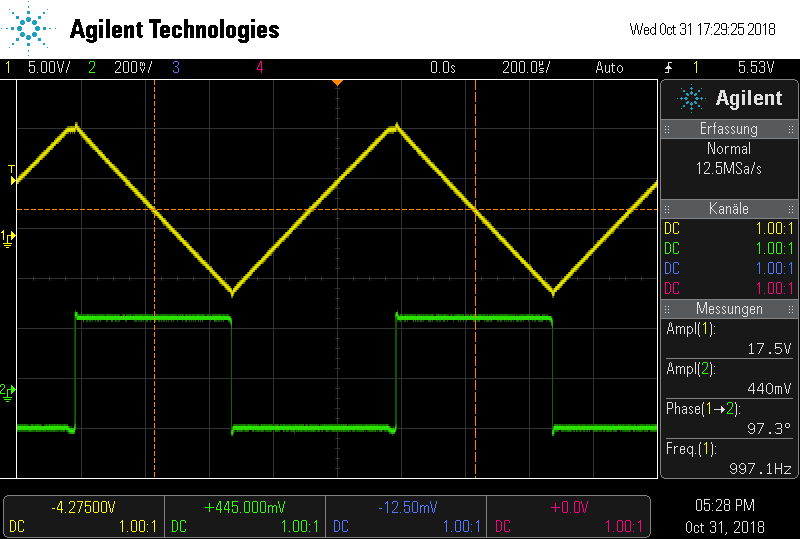
\includegraphics[scale=0.4]{scope_2.png}
  \caption{Integral of square-wave-voltage. Output (yellow line) and input (green line) of the integator circuit. The expectet integral relationship between the two wavesforms is evident.}
  \label{abb:3}
\end{figure}
\begin{figure}
  \centering
  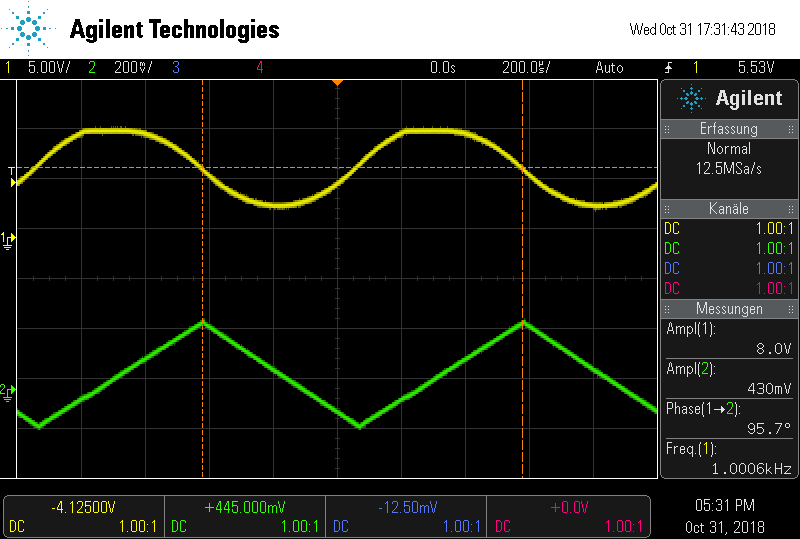
\includegraphics[scale=0.4]{scope_3.png}
  \caption{Integral of triangle-oscillation. Output (yellow line) and input (green line) of the integator circuit. The expectet integral relationship between the two wavesforms is evident.}
  \label{abb:4}
\end{figure}
\begin{figure}
  \centering
  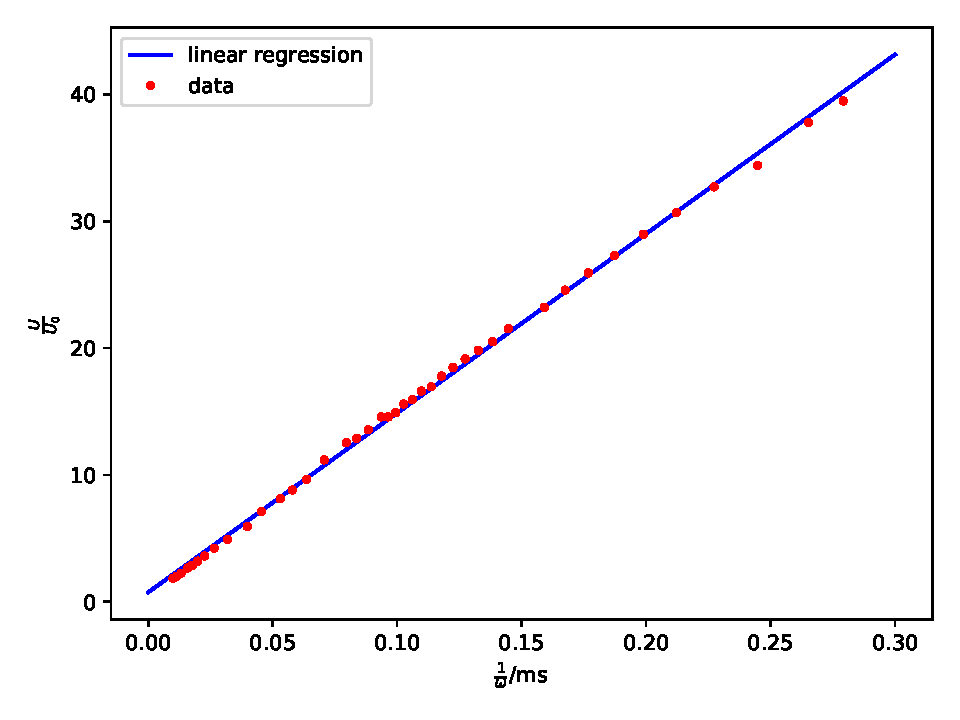
\includegraphics[scale=0.7]{3.pdf}
  \caption{The amplitude as a function of the inverse angular velocity.}
  \label{abb:5}
\end{figure}

\newpage
\subsection{Discussion}
In figures \ref{abb:1} and \ref{abb:2} the fall of the amplifier-factor is
visible very well and also the linear fit of the logarithm values.
The product of the constant amplifier-factor and the cut off frequency
should be a constant value. Here you can see, that it is in the same magnitude,
but just different:
\begin{align*}
  V_{0, 1} \cdot \nu_{\symup{g,1}} = \SI{0.9(5)}{\mega\hertz} \\
  V_{0, 2} \cdot \nu_{\symup{g,2}} = \SI{2.9(8)}{\mega\hertz}
\end{align*}
We cannot give a statement if this value is constant, because we did just two
measurements, but need more to obtain a significant result.

Out of the data of the amplitude as a function of the frequency you get the
value of the $RC$-member:

\begin{align*}
  RC = \SI{7.08(4)e-6}{\farad\ohm} \\
  RC_{theory}= \SI{6.15e-6}{\farad\ohm}
\end{align*}

It is a deviation of \SI{15}{\percent}. The big deviation can be based on
the inexact measurement of the capacity or the resistance.
In figures \ref{abb:3} and \ref{abb:4} you can see the integration of two
differenst voltage-shapes. As expected, the integral of a square-wave-voltage is an
triangle-oscillation and the integral of the triangle-oscillation is an
parabolic-oscillation.



\printbibliography
